%%%%%%%%%%%%%%%%%%%%%%%%%%%%%%%%%%%%%%%%%%%%%%%%%%
% Metadata
%%%%%%%%%%%%%%%%%%%%%%%%%%%%%%%%%%%%%%%%%%%%%%%%%%
% id: 2026-kyoto-5
% title: 2026年 京都大学 理系 第5問
% tags: []
% difficulty: C
% source: https://www.kyoto-u.ac.jp/sites/default/files/inline-files/admissionsundergradpast_eqR06_eqdocumentsR06_3M07-b3308c56005228b7b6d1c7e90375f55a.pdf

%%%%%%%%%%%%%%%%%%%%%%%%%%%%%%%%%%%%%%%%%%%%%%%%%%
% Preamble
%%%%%%%%%%%%%%%%%%%%%%%%%%%%%%%%%%%%%%%%%%%%%%%%%%
\documentclass[fleqn]{ltjsarticle}

\usepackage{common}
\loadcommonpreamble

% ヘッダー
\lhead{\textbf{2026年 京都大学 理系}}

%%%%%%%%%%%%%%%%%%%%%%%%%%%%%%%%%%%%%%%%%%%%%%%%%%
% Document
%%%%%%%%%%%%%%%%%%%%%%%%%%%%%%%%%%%%%%%%%%%%%%%%%%
\begin{document}

\begin{problembox}
    \begin{enumerate} 
        \item [\huge \shikakugo]\hfill\raisebox{1ex}{(35点)} \\
        $a$は$0<a<\pi$を満たす実数とする.$2$つの函数$y=\sin(x+a)$と$y=\sin(x-a)$のグラフの,$-\bunsuu\pi2\leqq x\leqq\bunsuu\pi2$の部分が囲む領域を$D_a$とする.$x$軸のまわりに$D_a$を$1$回転してできる立体の体積を求めよ.
    \end{enumerate}
\end{problembox}

\noindent
$0<a<\pi$および$-\bunsuu\pi2<x<\bunsuu\pi2$においては$\sin(x+a)-\sin(x-a)=2\cos x\sin a>0$が成り立つ.
\begin{enumerate}
\item[\tokeiichi]$0\leqq a\leqq\bunsuu\pi2$のとき\\
$-\bunsuu\pi2\leqq x\leqq-a$で$\sin(x+a)\leqq0$であり,$-a\leqq x\leqq\bunsuu\pi2$で$0\leqq\sin(x+a)$である.また,$-\bunsuu\pi2\leqq x\leqq a$で$\sin(x-a)\leqq0$であり,$a\leqq x\leqq\bunsuu\pi2$で$0\leqq\sin(x-a)$である.また,
\begin{align*}
\sin(x+a)+\sin(x-a)=2\sin x\cos a
\end{align*}
の符号は$x$の符号と一致するので,$-a\leqq x\leqq0$では$|\sin(x+a)|\leqq|\sin(x-a)|$であり,$0\leqq x\leqq a$では$|\sin(x-a)|\leqq|\sin(x+a)|$である.よって,領域$D_a$は以下のようになる.
$$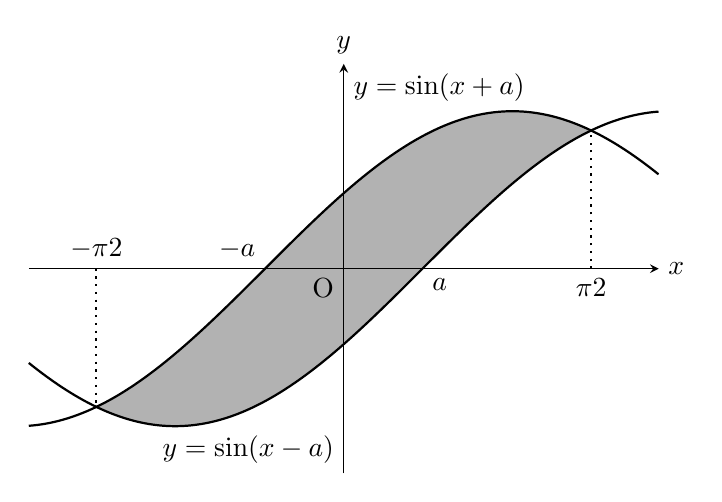
\begin{tikzpicture}[scale=2,samples=360]
\draw[-stealth](-2,0)--(2,0)node[right]{$x$};
\draw[-stealth](0,-1.3)--(0,1.3)node[above]{$y$};
\node at(0,0)[below left]{$\mathrm O$};
\fill[opacity=0.3,domain=-pi/2:pi/2]plot(\x,{sin((\x+0.5) r)})--plot(-\x,{sin((-\x-0.5) r)})--cycle;
\draw[thick,domain=-2:2]plot(\x,{sin((\x+0.5) r)});
\draw[thick,domain=-2:2]plot(\x,{sin((\x-0.5) r)});
\draw[thick,dotted](-pi/2,0)node[above]{$-\bunsuu\pi2$}--(-pi/2,{-cos(0.5 r)});
\draw[thick,dotted](pi/2,0)node[below]{$\bunsuu\pi2$}--(pi/2,{cos(0.5 r)});
\node at(-0.5,0)[above left]{$-a$};
\node at(0.5,0)[below right]{$a$};
\node at(0,1)[above right]{$y=\sin(x+a)$};
\node at(0,-1)[below left]{$y=\sin(x-a)$};
\end{tikzpicture}$$
$\sin((-x)+a)=-\sin(x-a)$であることから領域$D_a$は原点に関して点対称なので,求める体積$V$は$D_a$の$0<x$の範囲を回転させて得られる立体の体積の$2$倍である.よって
\begin{align*}
V&=2\left(\pi\int_0^{\pi/2}\sin^2(x+a)dx-\pi\int_a^{\pi/2}\sin^2(x-a)dx\right)\\
&=\pi\left(\int_0^{\pi/2}\Bigl(1-\cos(2(x+a))\Bigr)dx-\int_a^{\pi/2}\Bigl(1-\cos(2(x-a))\Bigr)dx\right)\\
&=\pi\left(\left[x-\bunsuu12\sin(2(x+a))\right]_0^{\pi/2}-\left[x-\bunsuu12\sin(2(x-a))\right]_a^{\pi/2}\right)\\
&=\pi\left(\bunsuu\pi2-\bunsuu12\sin(\pi+2a)+\bunsuu12\sin(2a)\right)-\pi\left(\bunsuu\pi2-\bunsuu12\sin(\pi-2a)+\bunsuu12\sin(-2a)\right)\\
&=\bunsuu\pi2\sin2a+\bunsuu\pi2\sin2a+\bunsuu\pi2\sin2a+\bunsuu\pi2\sin2a\\
&=2\pi\sin2a
\end{align*}
となる.
\item[\tokeini]$\bunsuu\pi2\leqq a\leqq\pi$のとき\\
各函数の符号および大小を\tokeiichi と同様に調べると,領域$D_a$は以下のようになる.
$$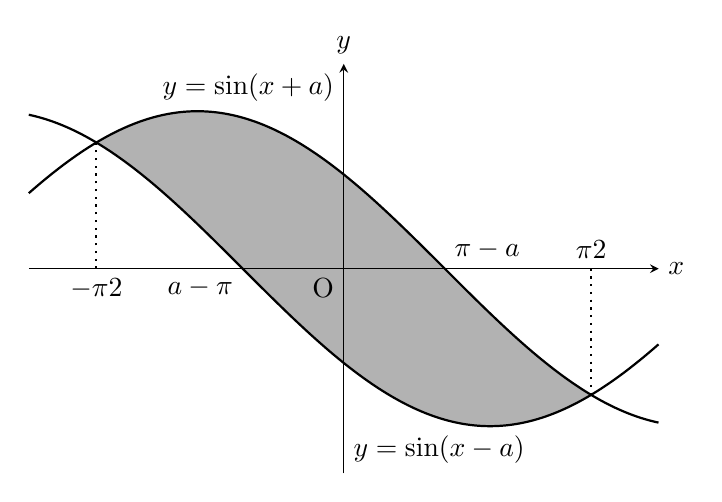
\begin{tikzpicture}[scale=2,samples=360]
\draw[-stealth](-2,0)--(2,0)node[right]{$x$};
\draw[-stealth](0,-1.3)--(0,1.3)node[above]{$y$};
\node at(0,0)[below left]{$\mathrm O$};
\fill[opacity=0.3,domain=-pi/2:pi/2]plot(\x,{sin((\x+2.5) r)})--plot(-\x,{sin((-\x-2.5) r)})--cycle;
\draw[thick,domain=-2:2]plot(\x,{sin((\x+2.5) r)});
\draw[thick,domain=-2:2]plot(\x,{sin((\x-2.5) r)});
\draw[thick,dotted](-pi/2,0)node[below]{$-\bunsuu\pi2$}--(-pi/2,{-cos(2.5 r)});
\draw[thick,dotted](pi/2,0)node[above]{$\bunsuu\pi2$}--(pi/2,{cos(2.5 r)});
\node at(2.5-pi,0)[below left]{$a-\pi$};
\node at(pi-2.5,0)[above right]{$\pi-a$};
\node at(0,1)[above left]{$y=\sin(x+a)$};
\node at(0,-1)[below right]{$y=\sin(x-a)$};
\end{tikzpicture}$$
\tokeiichi と同様の対称性から,求める体積$V$は
\begin{align*}
V&=2\left(\pi\int_0^{\pi/2}\sin^2(x-a)dx-\pi\int_a^{\pi/2}\sin^2(x+a)dx\right)\\
&=\pi\left(\int_0^{\pi/2}\Bigl(1-\cos(2(x-a))\Bigr)dx-\int_a^{\pi/2}\Bigl(1-\cos(2(x+a))\Bigr)dx\right)\\
&=\pi\left(\left[x-\bunsuu12\sin(2(x-a))\right]_0^{\pi/2}-\left[x-\bunsuu12\sin(2(x+a))\right]_a^{\pi/2}\right)\\
&=\pi\left(\bunsuu\pi2-\bunsuu12\sin(\pi-2a)+\bunsuu12\sin(-2a)\right)-\pi\left(\bunsuu\pi2-\bunsuu12\sin(\pi+2a)+\bunsuu12\sin(2a)\right)\\
&=-\bunsuu\pi2\sin2a-\bunsuu\pi2\sin2a-\bunsuu\pi2\sin2a-\bunsuu\pi2\sin2a\\
&=-2\pi\sin2a
\end{align*}
となる.
\end{enumerate}
\tokeiichi, \tokeini をまとめると,求める体積は$2\pi|\sin2a|$であることが分かる.

\end{document}